\documentclass[]{article}
\usepackage{lmodern}
\usepackage{amssymb,amsmath}
\usepackage{ifxetex,ifluatex}
\usepackage{fixltx2e} % provides \textsubscript
\ifnum 0\ifxetex 1\fi\ifluatex 1\fi=0 % if pdftex
  \usepackage[T1]{fontenc}
  \usepackage[utf8]{inputenc}
\else % if luatex or xelatex
  \ifxetex
    \usepackage{mathspec}
  \else
    \usepackage{fontspec}
  \fi
  \defaultfontfeatures{Ligatures=TeX,Scale=MatchLowercase}
\fi
% use upquote if available, for straight quotes in verbatim environments
\IfFileExists{upquote.sty}{\usepackage{upquote}}{}
% use microtype if available
\IfFileExists{microtype.sty}{%
\usepackage{microtype}
\UseMicrotypeSet[protrusion]{basicmath} % disable protrusion for tt fonts
}{}
\usepackage[margin=1in]{geometry}
\usepackage{hyperref}
\hypersetup{unicode=true,
            pdftitle={Preliminary version of seedHealth package vignette v8},
            pdfborder={0 0 0},
            breaklinks=true}
\urlstyle{same}  % don't use monospace font for urls
\usepackage{color}
\usepackage{fancyvrb}
\newcommand{\VerbBar}{|}
\newcommand{\VERB}{\Verb[commandchars=\\\{\}]}
\DefineVerbatimEnvironment{Highlighting}{Verbatim}{commandchars=\\\{\}}
% Add ',fontsize=\small' for more characters per line
\usepackage{framed}
\definecolor{shadecolor}{RGB}{248,248,248}
\newenvironment{Shaded}{\begin{snugshade}}{\end{snugshade}}
\newcommand{\KeywordTok}[1]{\textcolor[rgb]{0.13,0.29,0.53}{\textbf{#1}}}
\newcommand{\DataTypeTok}[1]{\textcolor[rgb]{0.13,0.29,0.53}{#1}}
\newcommand{\DecValTok}[1]{\textcolor[rgb]{0.00,0.00,0.81}{#1}}
\newcommand{\BaseNTok}[1]{\textcolor[rgb]{0.00,0.00,0.81}{#1}}
\newcommand{\FloatTok}[1]{\textcolor[rgb]{0.00,0.00,0.81}{#1}}
\newcommand{\ConstantTok}[1]{\textcolor[rgb]{0.00,0.00,0.00}{#1}}
\newcommand{\CharTok}[1]{\textcolor[rgb]{0.31,0.60,0.02}{#1}}
\newcommand{\SpecialCharTok}[1]{\textcolor[rgb]{0.00,0.00,0.00}{#1}}
\newcommand{\StringTok}[1]{\textcolor[rgb]{0.31,0.60,0.02}{#1}}
\newcommand{\VerbatimStringTok}[1]{\textcolor[rgb]{0.31,0.60,0.02}{#1}}
\newcommand{\SpecialStringTok}[1]{\textcolor[rgb]{0.31,0.60,0.02}{#1}}
\newcommand{\ImportTok}[1]{#1}
\newcommand{\CommentTok}[1]{\textcolor[rgb]{0.56,0.35,0.01}{\textit{#1}}}
\newcommand{\DocumentationTok}[1]{\textcolor[rgb]{0.56,0.35,0.01}{\textbf{\textit{#1}}}}
\newcommand{\AnnotationTok}[1]{\textcolor[rgb]{0.56,0.35,0.01}{\textbf{\textit{#1}}}}
\newcommand{\CommentVarTok}[1]{\textcolor[rgb]{0.56,0.35,0.01}{\textbf{\textit{#1}}}}
\newcommand{\OtherTok}[1]{\textcolor[rgb]{0.56,0.35,0.01}{#1}}
\newcommand{\FunctionTok}[1]{\textcolor[rgb]{0.00,0.00,0.00}{#1}}
\newcommand{\VariableTok}[1]{\textcolor[rgb]{0.00,0.00,0.00}{#1}}
\newcommand{\ControlFlowTok}[1]{\textcolor[rgb]{0.13,0.29,0.53}{\textbf{#1}}}
\newcommand{\OperatorTok}[1]{\textcolor[rgb]{0.81,0.36,0.00}{\textbf{#1}}}
\newcommand{\BuiltInTok}[1]{#1}
\newcommand{\ExtensionTok}[1]{#1}
\newcommand{\PreprocessorTok}[1]{\textcolor[rgb]{0.56,0.35,0.01}{\textit{#1}}}
\newcommand{\AttributeTok}[1]{\textcolor[rgb]{0.77,0.63,0.00}{#1}}
\newcommand{\RegionMarkerTok}[1]{#1}
\newcommand{\InformationTok}[1]{\textcolor[rgb]{0.56,0.35,0.01}{\textbf{\textit{#1}}}}
\newcommand{\WarningTok}[1]{\textcolor[rgb]{0.56,0.35,0.01}{\textbf{\textit{#1}}}}
\newcommand{\AlertTok}[1]{\textcolor[rgb]{0.94,0.16,0.16}{#1}}
\newcommand{\ErrorTok}[1]{\textcolor[rgb]{0.64,0.00,0.00}{\textbf{#1}}}
\newcommand{\NormalTok}[1]{#1}
\usepackage{graphicx,grffile}
\makeatletter
\def\maxwidth{\ifdim\Gin@nat@width>\linewidth\linewidth\else\Gin@nat@width\fi}
\def\maxheight{\ifdim\Gin@nat@height>\textheight\textheight\else\Gin@nat@height\fi}
\makeatother
% Scale images if necessary, so that they will not overflow the page
% margins by default, and it is still possible to overwrite the defaults
% using explicit options in \includegraphics[width, height, ...]{}
\setkeys{Gin}{width=\maxwidth,height=\maxheight,keepaspectratio}
\IfFileExists{parskip.sty}{%
\usepackage{parskip}
}{% else
\setlength{\parindent}{0pt}
\setlength{\parskip}{6pt plus 2pt minus 1pt}
}
\setlength{\emergencystretch}{3em}  % prevent overfull lines
\providecommand{\tightlist}{%
  \setlength{\itemsep}{0pt}\setlength{\parskip}{0pt}}
\setcounter{secnumdepth}{0}
% Redefines (sub)paragraphs to behave more like sections
\ifx\paragraph\undefined\else
\let\oldparagraph\paragraph
\renewcommand{\paragraph}[1]{\oldparagraph{#1}\mbox{}}
\fi
\ifx\subparagraph\undefined\else
\let\oldsubparagraph\subparagraph
\renewcommand{\subparagraph}[1]{\oldsubparagraph{#1}\mbox{}}
\fi

%%% Use protect on footnotes to avoid problems with footnotes in titles
\let\rmarkdownfootnote\footnote%
\def\footnote{\protect\rmarkdownfootnote}

%%% Change title format to be more compact
\usepackage{titling}

% Create subtitle command for use in maketitle
\newcommand{\subtitle}[1]{
  \posttitle{
    \begin{center}\large#1\end{center}
    }
}

\setlength{\droptitle}{-2em}

  \title{Preliminary version of seedHealth package vignette v8}
    \pretitle{\vspace{\droptitle}\centering\huge}
  \posttitle{\par}
    \author{}
    \preauthor{}\postauthor{}
    \date{}
    \predate{}\postdate{}
  

\begin{document}
\maketitle

\subsubsection{Slides for ths section can be found
here:}\label{slides-for-ths-section-can-be-found-here}

\begin{itemize}
\tightlist
\item
  \href{PDFFiles/R\%20packages\%20seedHealth\%20and\%20INAprelim.pdf}{Intro
  to Networks in R}
\end{itemize}

\subsection{seedHealth package
applications}\label{seedhealth-package-applications}

This package provides a scenario analysis for evaluating outcomes for
integrated seed health strategies. It is based on and builds on the
analyses and code from

Thomas-Sharma, S., Andrade-Piedra, J., Carvajal Yepes, M., Hernandez
Nopsa, J., Jeger, M., Jones, R., Kromann, P., Legg, J., Yuen, J.,
Forbes, G., and Garrett, K. A. 2017. A risk assessment framework for
seed degeneration: Informing an integrated seed health strategy for
vegetatively-propagated crops. Phytopathology 107:1123-1135.

Open access link for paper:
\url{https://apsjournals.apsnet.org/doi/10.1094/PHYTO-09-16-0340-R}

Link for online Shiny interface for exploring the seedHealth model:
\url{https://yanru-xing.shinyapps.io/SDAppvX1/}

\section{Getting the seedHealth package from
GitHub}\label{getting-the-seedhealth-package-from-github}

\begin{Shaded}
\begin{Highlighting}[]
\CommentTok{# this is a temporary fix to avoid possible error message, "trying to use CRAN without setting a mirror"}
\KeywordTok{options}\NormalTok{(}\DataTypeTok{repos=}\KeywordTok{structure}\NormalTok{(}\KeywordTok{c}\NormalTok{(}\DataTypeTok{CRAN=}\StringTok{"https://cran.cnr.berkeley.edu/"}\NormalTok{)))}

\CommentTok{#install devtools (only necessary once - uncomment the following line if you have not installed it yet)}
\KeywordTok{install.packages}\NormalTok{(}\StringTok{"devtools"}\NormalTok{)}
\end{Highlighting}
\end{Shaded}

\begin{verbatim}
## 
##   There is a binary version available but the source version is
##   later:
##          binary source needs_compilation
## devtools 1.13.6  2.0.1             FALSE
\end{verbatim}

\begin{verbatim}
## installing the source package 'devtools'
\end{verbatim}

\begin{Shaded}
\begin{Highlighting}[]
\KeywordTok{library}\NormalTok{(devtools)}

\CommentTok{# use devtools function install_github to install the seedHealth version available on GitHub}
\CommentTok{# this is only necessary once, until a new version is available}
\CommentTok{# uncomment the following line if you have not installed seedHealth yet, or a new version is available}

\CommentTok{#devtools::install_github("GarrettLab/seedHealth")}

\KeywordTok{library}\NormalTok{(seedHealth)}
\end{Highlighting}
\end{Shaded}

The code below uses two other R packages - these will need to be
installed if they have not yet been installed. The commands for
installing are commented out below, but the ``\#'' in front of the
command line can be removed to install.

\section{Function onesim}\label{function-onesim}

This function evaluates a time series of yield loss due to seed
degeneration across seasons. Weather conduciveness to disease and other
factors are included as stochastic components of the model.

\section{Arguments in function
onesim}\label{arguments-in-function-onesim}

There are several arguments that can be modified in function onesim to
describe how seed degeneration occurs over time. These arguments are
described in more detail in a table in Thomas-Sharma et al. 2017.

pHSinit the initial proportion of healthy seed, numeric or numeric
vector. Kx\\
the total number of plants, positive interger, numeric or numeric
vector. betax\\
the maximum seasonal transmission rate, numeric or numeric vector.
wxtnormm\\
the environmental effect on transmission rate (mean of underlying normal
distribution prior to truncation), numeric or numeric vector.
wxtnormsd\\
the environmental effect on transmission rate (standard deviation of
underlying normal distribution prior to truncation), numeric or numeric
vector. hx\\
the host effect on transmission rate, numeric or numeric vector.
mxtnormm\\
the vector management effect on transmission rate (mean of underlying
normal distribution prior to truncation), numeric or numeric vector.
mxtnormsd\\
the vector management effect on transmission rate (standard deviation of
underlying normal distribution prior to truncation), numeric or numeric
vector. axtnormm\\
the roguing effect in terms of decreased DP (mean of underlying normal
distribution prior to truncation), numeric or numeric vector.
axtnormsd\\
the roguing effect in terms of decreased DP (standard deviation of
underlying normal distribution prior to truncation), numeric or numeric
vector. rx\\
the reversion rate, numeric or numeric vector. zxtnormm\\
the proportional selection against diseased plants (mean of underlying
normal distribution prior to truncation), numeric or numeric vector.
zxtnormsd\\
the proportional selection against diseased plants (standard deviation
of underlying normal distribution prior to truncation), numeric or
numeric vector. gx\\
the seed production rate in healthy plants, numeric or numeric vector.
cx\\
the proportional seed production rate in diseased plants, numeric or
numeric vector. phix\\
the proportion clean seed purchased, numeric or numeric vector.
nseasons\\
the number of seasons, numeric or numeric vector. HPcut\\
the proportion healthy plant number cutoff, numeric or numeric vector.
pHScut\\
the proportion healthy seed cutoff, numeric or numeric vector. maY the
maximum attainable yield, end of season, in the absence of disease,
numeric or numeric vector. miY the minimum yield when all plants are
diseased (useable yield despite disease), numeric or numeric vector.
thetax\\
the rate of decline of Yld with increasing disease incidence, numeric or
numeric vector. Ex\\
the amount of external inoculum around field, numeric or numeric vector.

\subsection{Example of plotting seed degeneration effects over
time}\label{example-of-plotting-seed-degeneration-effects-over-time}

Note that this command produces results similar to those from the online
Shiny interface for seedHealth

\begin{Shaded}
\begin{Highlighting}[]
\KeywordTok{install.packages}\NormalTok{(}\StringTok{"RColorBrewer"}\NormalTok{) }\CommentTok{# remove the initial '#' if this is not yet installed}
\end{Highlighting}
\end{Shaded}

\begin{verbatim}
## 
## The downloaded binary packages are in
##  /var/folders/3f/wdpyyh2x0r5c5j0s55mwx8d80000gn/T//RtmpMzdLPm/downloaded_packages
\end{verbatim}

\begin{Shaded}
\begin{Highlighting}[]
\KeywordTok{library}\NormalTok{(RColorBrewer)}

\NormalTok{out1 <-}\StringTok{ }\KeywordTok{onesim}\NormalTok{(}\DataTypeTok{pHSinit=}\FloatTok{0.8}\NormalTok{, }\DataTypeTok{Kx =} \DecValTok{100}\NormalTok{, }\DataTypeTok{betax=}\FloatTok{0.02}\NormalTok{, }\DataTypeTok{wxtnormm=}\FloatTok{0.8}\NormalTok{, }\DataTypeTok{wxtnormsd=} \FloatTok{0.1}\NormalTok{, }\DataTypeTok{hx=}\DecValTok{1}\NormalTok{, }\DataTypeTok{mxtnormm=}\DecValTok{1}\NormalTok{, }\DataTypeTok{mxtnormsd=}\DecValTok{0}\NormalTok{, }\DataTypeTok{axtnormm=}\DecValTok{1}\NormalTok{, }\DataTypeTok{axtnormsd=}\DecValTok{0}\NormalTok{, }\DataTypeTok{rx=}\FloatTok{0.1}\NormalTok{, }\DataTypeTok{zxtnormm=}\DecValTok{1}\NormalTok{, }\DataTypeTok{zxtnormsd=} \DecValTok{0}\NormalTok{, }\DataTypeTok{gx=}\DecValTok{4}\NormalTok{,}\DataTypeTok{cx=}\FloatTok{0.9}\NormalTok{, }\DataTypeTok{phix=}\DecValTok{0}\NormalTok{, }\DataTypeTok{nseasons=}\DecValTok{10}\NormalTok{, }\DataTypeTok{HPcut=}\FloatTok{0.5}\NormalTok{, }\DataTypeTok{pHScut=}\FloatTok{0.5}\NormalTok{,}\DataTypeTok{maY=}\DecValTok{100}\NormalTok{,}\DataTypeTok{miY=}\DecValTok{0}\NormalTok{,}\DataTypeTok{thetax=}\FloatTok{0.2}\NormalTok{, }\DataTypeTok{Ex=}\DecValTok{0}\NormalTok{)}
\NormalTok{int1 <-}\StringTok{ }\NormalTok{out1}\OperatorTok{$}\NormalTok{outm}\OperatorTok{$}\NormalTok{YL}
\NormalTok{seas1 <-}\StringTok{ }\NormalTok{out1}\OperatorTok{$}\NormalTok{outm}\OperatorTok{$}\NormalTok{season}

\CommentTok{# nreals is the number of realizations - higher values gives a smoother plot}
\NormalTok{nreals <-}\StringTok{ }\DecValTok{10}

\ControlFlowTok{for}\NormalTok{(i }\ControlFlowTok{in} \DecValTok{1}\OperatorTok{:}\NormalTok{nreals)\{ }
\NormalTok{    out1 <-}\StringTok{ }\KeywordTok{onesim}\NormalTok{(}\DataTypeTok{pHSinit=}\FloatTok{0.8}\NormalTok{, }\DataTypeTok{Kx =} \DecValTok{100}\NormalTok{, }\DataTypeTok{betax=}\FloatTok{0.02}\NormalTok{, }\DataTypeTok{wxtnormm=}\FloatTok{0.8}\NormalTok{, }\DataTypeTok{wxtnormsd=} \FloatTok{0.1}\NormalTok{, }\DataTypeTok{hx=}\DecValTok{1}\NormalTok{, }\DataTypeTok{mxtnormm=}\DecValTok{1}\NormalTok{, }\DataTypeTok{mxtnormsd=}\DecValTok{0}\NormalTok{, }\DataTypeTok{axtnormm=}\DecValTok{1}\NormalTok{, }\DataTypeTok{axtnormsd=}\DecValTok{0}\NormalTok{, }\DataTypeTok{rx=}\FloatTok{0.1}\NormalTok{, }\DataTypeTok{zxtnormm=}\DecValTok{1}\NormalTok{, }\DataTypeTok{zxtnormsd=} \DecValTok{0}\NormalTok{, }\DataTypeTok{gx=}\DecValTok{4}\NormalTok{,}\DataTypeTok{cx=}\FloatTok{0.9}\NormalTok{, }\DataTypeTok{phix=}\DecValTok{0}\NormalTok{, }\DataTypeTok{nseasons=}\DecValTok{10}\NormalTok{, }\DataTypeTok{HPcut=}\FloatTok{0.5}\NormalTok{, }\DataTypeTok{pHScut=}\FloatTok{0.5}\NormalTok{,}\DataTypeTok{maY=}\DecValTok{100}\NormalTok{,}\DataTypeTok{miY=}\DecValTok{0}\NormalTok{,}\DataTypeTok{thetax=}\FloatTok{0.2}\NormalTok{, }\DataTypeTok{Ex=}\DecValTok{0}\NormalTok{)}
\NormalTok{    int1 <-}\StringTok{ }\KeywordTok{rbind}\NormalTok{(int1,out1}\OperatorTok{$}\NormalTok{outm}\OperatorTok{$}\NormalTok{YL)}
\NormalTok{    seas1 <-}\StringTok{ }\KeywordTok{rbind}\NormalTok{(seas1,out1}\OperatorTok{$}\NormalTok{outm}\OperatorTok{$}\NormalTok{season)}
\NormalTok{\}}

\KeywordTok{smoothScatter}\NormalTok{(seas1,int1, }\DataTypeTok{xlab=}\StringTok{''}\NormalTok{, }\DataTypeTok{ylab=}\StringTok{'Yield loss (%)'}\NormalTok{,}\DataTypeTok{ylim=}\KeywordTok{c}\NormalTok{(}\DecValTok{0}\NormalTok{,}\DecValTok{100}\NormalTok{), }\DataTypeTok{font.lab=}\DecValTok{2}\NormalTok{, }\DataTypeTok{cex.lab=}\FloatTok{1.5}\NormalTok{, }\DataTypeTok{cex.axis=}\FloatTok{1.25}\NormalTok{, }\DataTypeTok{nrpoints=}\DecValTok{0}\NormalTok{, }\DataTypeTok{colramp=}\KeywordTok{colorRampPalette}\NormalTok{(}\KeywordTok{brewer.pal}\NormalTok{(}\DecValTok{8}\NormalTok{,}\StringTok{"Greys"}\NormalTok{)))}
\KeywordTok{lines}\NormalTok{(}\KeywordTok{colMeans}\NormalTok{(seas1), }\KeywordTok{colMeans}\NormalTok{(int1), }\DataTypeTok{type=}\StringTok{'l'}\NormalTok{, }\DataTypeTok{col=}\StringTok{'red'}\NormalTok{)}
\end{Highlighting}
\end{Shaded}

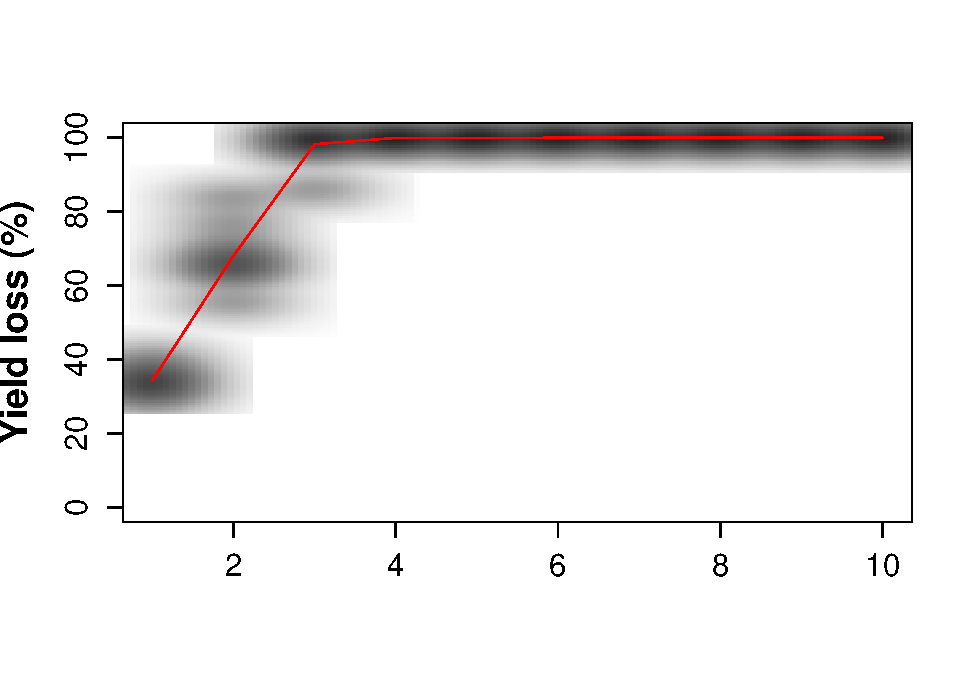
\includegraphics{seedHealth_files/figure-latex/unnamed-chunk-2-1.pdf}

\begin{Shaded}
\begin{Highlighting}[]
\CommentTok{# Could produce a summary table}
\CommentTok{#write.table(x=int1, file=paste('int_out1','csv', sep='.'), sep=',',append=F, row.names=FALSE)}
\end{Highlighting}
\end{Shaded}

\subsection{Fig. 2. from Thomas-Sharma et al. 2017: Long-term yield loss
under no management
scenarios}\label{fig.-2.-from-thomas-sharma-et-al.-2017-long-term-yield-loss-under-no-management-scenarios}

\begin{Shaded}
\begin{Highlighting}[]
\KeywordTok{par}\NormalTok{(}\DataTypeTok{mfrow=}\KeywordTok{c}\NormalTok{(}\DecValTok{2}\NormalTok{,}\DecValTok{2}\NormalTok{), }\DataTypeTok{mar=}\KeywordTok{c}\NormalTok{(}\DecValTok{4}\NormalTok{,}\FloatTok{4.4}\NormalTok{,}\FloatTok{0.5}\NormalTok{,}\FloatTok{0.5}\NormalTok{), }\DataTypeTok{oma=}\KeywordTok{c}\NormalTok{(}\FloatTok{0.5}\NormalTok{,}\FloatTok{0.5}\NormalTok{,}\FloatTok{0.25}\NormalTok{,}\FloatTok{0.25}\NormalTok{))}

\NormalTok{out1 <-}\StringTok{ }\KeywordTok{onesim}\NormalTok{(}\DataTypeTok{pHSinit=}\FloatTok{0.8}\NormalTok{, }\DataTypeTok{Kx =} \DecValTok{100}\NormalTok{, }\DataTypeTok{betax=}\FloatTok{0.02}\NormalTok{, }\DataTypeTok{wxtnormm=}\FloatTok{0.8}\NormalTok{, }\DataTypeTok{wxtnormsd=} \FloatTok{0.1}\NormalTok{, }\DataTypeTok{hx=}\DecValTok{1}\NormalTok{, }\DataTypeTok{mxtnormm=}\DecValTok{1}\NormalTok{, }\DataTypeTok{mxtnormsd=}\DecValTok{0}\NormalTok{, }\DataTypeTok{axtnormm=}\DecValTok{1}\NormalTok{, }\DataTypeTok{axtnormsd=}\DecValTok{0}\NormalTok{, }\DataTypeTok{rx=}\FloatTok{0.1}\NormalTok{, }\DataTypeTok{zxtnormm=}\DecValTok{1}\NormalTok{, }\DataTypeTok{zxtnormsd=} \DecValTok{0}\NormalTok{, }\DataTypeTok{gx=}\DecValTok{4}\NormalTok{,}\DataTypeTok{cx=}\FloatTok{0.9}\NormalTok{, }\DataTypeTok{phix=}\DecValTok{0}\NormalTok{, }\DataTypeTok{nseasons=}\DecValTok{10}\NormalTok{, }\DataTypeTok{HPcut=}\FloatTok{0.5}\NormalTok{, }\DataTypeTok{pHScut=}\FloatTok{0.5}\NormalTok{,}\DataTypeTok{maY=}\DecValTok{100}\NormalTok{,}\DataTypeTok{miY=}\DecValTok{0}\NormalTok{,}\DataTypeTok{thetax=}\FloatTok{0.2}\NormalTok{, }\DataTypeTok{Ex=}\DecValTok{0}\NormalTok{)}
\NormalTok{int1 <-}\StringTok{ }\NormalTok{out1}\OperatorTok{$}\NormalTok{outm}\OperatorTok{$}\NormalTok{YL}
\NormalTok{seas1 <-}\StringTok{ }\NormalTok{out1}\OperatorTok{$}\NormalTok{outm}\OperatorTok{$}\NormalTok{season}

\CommentTok{# temporary note: wxd and wdsamp were removed}

\CommentTok{# nreals is the number of realizations - higher values gives a smoother plot}
\NormalTok{nreals <-}\StringTok{ }\DecValTok{10}

\ControlFlowTok{for}\NormalTok{(i }\ControlFlowTok{in} \DecValTok{1}\OperatorTok{:}\NormalTok{nreals)\{ }
\NormalTok{    out1 <-}\StringTok{ }\KeywordTok{onesim}\NormalTok{(}\DataTypeTok{pHSinit=}\FloatTok{0.8}\NormalTok{, }\DataTypeTok{Kx =} \DecValTok{100}\NormalTok{, }\DataTypeTok{betax=}\FloatTok{0.02}\NormalTok{, }\DataTypeTok{wxtnormm=}\FloatTok{0.8}\NormalTok{, }\DataTypeTok{wxtnormsd=} \FloatTok{0.1}\NormalTok{, }\DataTypeTok{hx=}\DecValTok{1}\NormalTok{, }\DataTypeTok{mxtnormm=}\DecValTok{1}\NormalTok{, }\DataTypeTok{mxtnormsd=}\DecValTok{0}\NormalTok{, }\DataTypeTok{axtnormm=}\DecValTok{1}\NormalTok{, }\DataTypeTok{axtnormsd=}\DecValTok{0}\NormalTok{, }\DataTypeTok{rx=}\FloatTok{0.1}\NormalTok{, }\DataTypeTok{zxtnormm=}\DecValTok{1}\NormalTok{, }\DataTypeTok{zxtnormsd=} \DecValTok{0}\NormalTok{, }\DataTypeTok{gx=}\DecValTok{4}\NormalTok{,}\DataTypeTok{cx=}\FloatTok{0.9}\NormalTok{, }\DataTypeTok{phix=}\DecValTok{0}\NormalTok{, }\DataTypeTok{nseasons=}\DecValTok{10}\NormalTok{, }\DataTypeTok{HPcut=}\FloatTok{0.5}\NormalTok{, }\DataTypeTok{pHScut=}\FloatTok{0.5}\NormalTok{,}\DataTypeTok{maY=}\DecValTok{100}\NormalTok{,}\DataTypeTok{miY=}\DecValTok{0}\NormalTok{,}\DataTypeTok{thetax=}\FloatTok{0.2}\NormalTok{, }\DataTypeTok{Ex=}\DecValTok{0}\NormalTok{)}
\NormalTok{    int1 <-}\StringTok{ }\KeywordTok{rbind}\NormalTok{(int1,out1}\OperatorTok{$}\NormalTok{outm}\OperatorTok{$}\NormalTok{YL)}
\NormalTok{    seas1 <-}\StringTok{ }\KeywordTok{rbind}\NormalTok{(seas1,out1}\OperatorTok{$}\NormalTok{outm}\OperatorTok{$}\NormalTok{season)}
\NormalTok{\}}

\CommentTok{# Could produce an about table}
\CommentTok{# write.table(x=int1, file=paste('int_out1','csv', sep='.'), sep=',',append=F, row.names=FALSE)}

\KeywordTok{smoothScatter}\NormalTok{(seas1,int1, }\DataTypeTok{xlab=}\StringTok{''}\NormalTok{, }\DataTypeTok{ylab=}\StringTok{'Yield loss (%)'}\NormalTok{,}\DataTypeTok{ylim=}\KeywordTok{c}\NormalTok{(}\DecValTok{0}\NormalTok{,}\DecValTok{100}\NormalTok{), }\DataTypeTok{font.lab=}\DecValTok{2}\NormalTok{, }\DataTypeTok{cex.lab=}\FloatTok{1.5}\NormalTok{, }\DataTypeTok{cex.axis=}\FloatTok{1.25}\NormalTok{, }\DataTypeTok{nrpoints=}\DecValTok{0}\NormalTok{, }\DataTypeTok{colramp=}\KeywordTok{colorRampPalette}\NormalTok{(}\KeywordTok{brewer.pal}\NormalTok{(}\DecValTok{8}\NormalTok{,}\StringTok{"Greys"}\NormalTok{)))}
\KeywordTok{lines}\NormalTok{(}\KeywordTok{colMeans}\NormalTok{(seas1), }\KeywordTok{colMeans}\NormalTok{(int1), }\DataTypeTok{type=}\StringTok{'l'}\NormalTok{, }\DataTypeTok{col=}\StringTok{'red'}\NormalTok{)}

\NormalTok{out2 <-}\StringTok{ }\KeywordTok{onesim}\NormalTok{(}\DataTypeTok{pHSinit=}\FloatTok{0.8}\NormalTok{, }\DataTypeTok{Kx =} \DecValTok{100}\NormalTok{, }\DataTypeTok{betax=}\FloatTok{0.02}\NormalTok{, }\DataTypeTok{wxtnormm=}\FloatTok{0.8}\NormalTok{, }\DataTypeTok{wxtnormsd=} \FloatTok{0.3}\NormalTok{, }\DataTypeTok{hx=}\DecValTok{1}\NormalTok{, }\DataTypeTok{mxtnormm=}\DecValTok{1}\NormalTok{, }\DataTypeTok{mxtnormsd=}\DecValTok{0}\NormalTok{, }\DataTypeTok{axtnormm=}\DecValTok{1}\NormalTok{, }\DataTypeTok{axtnormsd=}\DecValTok{0}\NormalTok{, }\DataTypeTok{rx=}\FloatTok{0.1}\NormalTok{, }\DataTypeTok{zxtnormm=}\DecValTok{1}\NormalTok{, }\DataTypeTok{zxtnormsd=} \DecValTok{0}\NormalTok{,}\DataTypeTok{gx=}\DecValTok{4}\NormalTok{,}\DataTypeTok{cx=}\FloatTok{0.9}\NormalTok{, }\DataTypeTok{phix=}\DecValTok{0}\NormalTok{, }\DataTypeTok{nseasons=}\DecValTok{10}\NormalTok{, }\DataTypeTok{HPcut=}\FloatTok{0.5}\NormalTok{, }\DataTypeTok{pHScut=}\FloatTok{0.5}\NormalTok{,}\DataTypeTok{maY=}\DecValTok{100}\NormalTok{,}\DataTypeTok{miY=}\DecValTok{0}\NormalTok{,}\DataTypeTok{thetax=}\FloatTok{0.2}\NormalTok{, }\DataTypeTok{Ex=}\DecValTok{0}\NormalTok{)}
\NormalTok{int2 <-}\StringTok{ }\NormalTok{out2}\OperatorTok{$}\NormalTok{outm}\OperatorTok{$}\NormalTok{YL}
\NormalTok{seas2 <-}\StringTok{ }\NormalTok{out2}\OperatorTok{$}\NormalTok{outm}\OperatorTok{$}\NormalTok{season}

\CommentTok{# for speed, only "i in 1:10"}

\ControlFlowTok{for}\NormalTok{(i }\ControlFlowTok{in} \DecValTok{1}\OperatorTok{:}\NormalTok{nreals)\{ }\CommentTok{# higher values make a smoother plot}
\NormalTok{    out2 <-}\StringTok{ }\KeywordTok{onesim}\NormalTok{(}\DataTypeTok{pHSinit=}\FloatTok{0.8}\NormalTok{, }\DataTypeTok{Kx =} \DecValTok{100}\NormalTok{, }\DataTypeTok{betax=}\FloatTok{0.02}\NormalTok{, }\DataTypeTok{wxtnormm=}\FloatTok{0.8}\NormalTok{, }\DataTypeTok{wxtnormsd=} \FloatTok{0.3}\NormalTok{, }\DataTypeTok{hx=}\DecValTok{1}\NormalTok{, }\DataTypeTok{mxtnormm=}\DecValTok{1}\NormalTok{, }\DataTypeTok{mxtnormsd=}\DecValTok{0}\NormalTok{, }\DataTypeTok{axtnormm=}\DecValTok{1}\NormalTok{, }\DataTypeTok{axtnormsd=}\DecValTok{0}\NormalTok{, }\DataTypeTok{rx=}\FloatTok{0.1}\NormalTok{, }\DataTypeTok{zxtnormm=}\DecValTok{1}\NormalTok{, }\DataTypeTok{zxtnormsd=} \DecValTok{0}\NormalTok{, }\DataTypeTok{gx=}\DecValTok{4}\NormalTok{,}\DataTypeTok{cx=}\FloatTok{0.9}\NormalTok{, }\DataTypeTok{phix=}\DecValTok{0}\NormalTok{, }\DataTypeTok{nseasons=}\DecValTok{10}\NormalTok{, }\DataTypeTok{HPcut=}\FloatTok{0.5}\NormalTok{, }\DataTypeTok{pHScut=}\FloatTok{0.5}\NormalTok{,}\DataTypeTok{maY=}\DecValTok{100}\NormalTok{,}\DataTypeTok{miY=}\DecValTok{0}\NormalTok{, }\DataTypeTok{thetax=}\FloatTok{0.2}\NormalTok{, }\DataTypeTok{Ex=}\DecValTok{0}\NormalTok{)}
\NormalTok{    int2 <-}\StringTok{ }\KeywordTok{rbind}\NormalTok{(int2,out2}\OperatorTok{$}\NormalTok{outm}\OperatorTok{$}\NormalTok{YL)}
\NormalTok{    seas2 <-}\StringTok{ }\KeywordTok{rbind}\NormalTok{(seas2,out2}\OperatorTok{$}\NormalTok{outm}\OperatorTok{$}\NormalTok{season)}
\NormalTok{\}}

\CommentTok{#write.table(x=int2, file=paste('int_out2','csv', sep='.'), sep=',',append=F, row.names=FALSE)}

\KeywordTok{smoothScatter}\NormalTok{(seas2,int2, }\DataTypeTok{xlab=}\StringTok{''}\NormalTok{, }\DataTypeTok{ylab=}\StringTok{''}\NormalTok{,}\DataTypeTok{ylim=}\KeywordTok{c}\NormalTok{(}\DecValTok{0}\NormalTok{,}\DecValTok{100}\NormalTok{), }\DataTypeTok{font.lab=}\DecValTok{2}\NormalTok{, }\DataTypeTok{cex.lab=}\FloatTok{1.5}\NormalTok{, }\DataTypeTok{cex.axis=}\FloatTok{1.25}\NormalTok{, }\DataTypeTok{nrpoints=}\DecValTok{0}\NormalTok{, }\DataTypeTok{colramp=}\KeywordTok{colorRampPalette}\NormalTok{(}\KeywordTok{brewer.pal}\NormalTok{(}\DecValTok{8}\NormalTok{,}\StringTok{"Greys"}\NormalTok{)))}
\KeywordTok{lines}\NormalTok{(}\KeywordTok{colMeans}\NormalTok{(seas2), }\KeywordTok{colMeans}\NormalTok{(int2), }\DataTypeTok{type=}\StringTok{'l'}\NormalTok{, }\DataTypeTok{col=}\StringTok{'red'}\NormalTok{)}

\NormalTok{out3 <-}\StringTok{ }\KeywordTok{onesim}\NormalTok{(}\DataTypeTok{pHSinit=}\FloatTok{0.8}\NormalTok{, }\DataTypeTok{Kx =} \DecValTok{100}\NormalTok{, }\DataTypeTok{betax=}\FloatTok{0.02}\NormalTok{, }\DataTypeTok{wxtnormm=}\FloatTok{0.2}\NormalTok{, }\DataTypeTok{wxtnormsd=} \FloatTok{0.1}\NormalTok{, }\DataTypeTok{hx=}\DecValTok{1}\NormalTok{, }\DataTypeTok{mxtnormm=}\DecValTok{1}\NormalTok{, }\DataTypeTok{mxtnormsd=}\DecValTok{0}\NormalTok{, }\DataTypeTok{axtnormm=}\DecValTok{1}\NormalTok{, }\DataTypeTok{axtnormsd=}\DecValTok{0}\NormalTok{, }\DataTypeTok{rx=}\FloatTok{0.1}\NormalTok{, }\DataTypeTok{zxtnormm=}\DecValTok{1}\NormalTok{, }\DataTypeTok{zxtnormsd=} \DecValTok{0}\NormalTok{, }\DataTypeTok{gx=}\DecValTok{4}\NormalTok{,}\DataTypeTok{cx=}\FloatTok{0.9}\NormalTok{, }\DataTypeTok{phix=}\DecValTok{0}\NormalTok{, }\DataTypeTok{nseasons=}\DecValTok{10}\NormalTok{, }\DataTypeTok{HPcut=}\FloatTok{0.5}\NormalTok{, }\DataTypeTok{pHScut=}\FloatTok{0.5}\NormalTok{,}\DataTypeTok{maY=}\DecValTok{100}\NormalTok{,}\DataTypeTok{miY=}\DecValTok{0}\NormalTok{,}\DataTypeTok{thetax=}\FloatTok{0.2}\NormalTok{, }\DataTypeTok{Ex=}\DecValTok{0}\NormalTok{)}
\NormalTok{int3 <-}\StringTok{ }\NormalTok{out3}\OperatorTok{$}\NormalTok{outm}\OperatorTok{$}\NormalTok{YL}
\NormalTok{seas3 <-}\StringTok{ }\NormalTok{out3}\OperatorTok{$}\NormalTok{outm}\OperatorTok{$}\NormalTok{season}


\ControlFlowTok{for}\NormalTok{(i }\ControlFlowTok{in} \DecValTok{1}\OperatorTok{:}\NormalTok{nreals)\{ }\CommentTok{# higher values make a smoother plot}
\NormalTok{    out3 <-}\StringTok{ }\KeywordTok{onesim}\NormalTok{(}\DataTypeTok{pHSinit=}\FloatTok{0.8}\NormalTok{, }\DataTypeTok{Kx =} \DecValTok{100}\NormalTok{, }\DataTypeTok{betax=}\FloatTok{0.02}\NormalTok{, }\DataTypeTok{wxtnormm=}\FloatTok{0.2}\NormalTok{, }\DataTypeTok{wxtnormsd=} \FloatTok{0.1}\NormalTok{, }\DataTypeTok{hx=}\DecValTok{1}\NormalTok{, }\DataTypeTok{mxtnormm=}\DecValTok{1}\NormalTok{, }\DataTypeTok{mxtnormsd=}\DecValTok{0}\NormalTok{, }\DataTypeTok{axtnormm=}\DecValTok{1}\NormalTok{, }\DataTypeTok{axtnormsd=}\DecValTok{0}\NormalTok{, }\DataTypeTok{rx=}\FloatTok{0.1}\NormalTok{, }\DataTypeTok{zxtnormm=}\DecValTok{1}\NormalTok{, }\DataTypeTok{zxtnormsd=} \DecValTok{0}\NormalTok{,}\DataTypeTok{gx=}\DecValTok{4}\NormalTok{,}\DataTypeTok{cx=}\FloatTok{0.9}\NormalTok{, }\DataTypeTok{phix=}\DecValTok{0}\NormalTok{, }\DataTypeTok{nseasons=}\DecValTok{10}\NormalTok{, }\DataTypeTok{HPcut=}\FloatTok{0.5}\NormalTok{, }\DataTypeTok{pHScut=}\FloatTok{0.5}\NormalTok{,}\DataTypeTok{maY=}\DecValTok{100}\NormalTok{,}\DataTypeTok{miY=}\DecValTok{0}\NormalTok{,}\DataTypeTok{thetax=}\FloatTok{0.2}\NormalTok{, }\DataTypeTok{Ex=}\DecValTok{0}\NormalTok{)}
\NormalTok{    int3 <-}\StringTok{ }\KeywordTok{rbind}\NormalTok{(int3,out3}\OperatorTok{$}\NormalTok{outm}\OperatorTok{$}\NormalTok{YL)}
\NormalTok{    seas3 <-}\StringTok{ }\KeywordTok{rbind}\NormalTok{(seas3,out3}\OperatorTok{$}\NormalTok{outm}\OperatorTok{$}\NormalTok{season)}
\NormalTok{\}}
\CommentTok{#write.table(x=int3, file=paste('int_out3','csv', sep='.'), sep=',',append=F, row.names=FALSE)}

\KeywordTok{smoothScatter}\NormalTok{(seas3,int3, }\DataTypeTok{xlab=}\StringTok{'Number of seasons'}\NormalTok{, }\DataTypeTok{ylab=}\StringTok{'Yield loss (%)'}\NormalTok{,}\DataTypeTok{ylim=}\KeywordTok{c}\NormalTok{(}\DecValTok{0}\NormalTok{,}\DecValTok{100}\NormalTok{), }\DataTypeTok{font.lab=}\DecValTok{2}\NormalTok{, }\DataTypeTok{cex.lab=}\FloatTok{1.5}\NormalTok{, }\DataTypeTok{cex.axis=}\FloatTok{1.25}\NormalTok{, }\DataTypeTok{nrpoints=}\DecValTok{0}\NormalTok{, }\DataTypeTok{colramp=}\KeywordTok{colorRampPalette}\NormalTok{(}\KeywordTok{brewer.pal}\NormalTok{(}\DecValTok{8}\NormalTok{,}\StringTok{"Greys"}\NormalTok{)))}
\KeywordTok{lines}\NormalTok{(}\KeywordTok{colMeans}\NormalTok{(seas3), }\KeywordTok{colMeans}\NormalTok{(int3), }\DataTypeTok{type=}\StringTok{'l'}\NormalTok{, }\DataTypeTok{col=}\StringTok{'red'}\NormalTok{)}

\NormalTok{out4 <-}\StringTok{ }\KeywordTok{onesim}\NormalTok{(}\DataTypeTok{pHSinit=}\FloatTok{0.8}\NormalTok{, }\DataTypeTok{Kx =} \DecValTok{100}\NormalTok{, }\DataTypeTok{betax=}\FloatTok{0.02}\NormalTok{, }\DataTypeTok{wxtnormm=}\FloatTok{0.2}\NormalTok{, }\DataTypeTok{wxtnormsd=} \FloatTok{0.3}\NormalTok{, }\DataTypeTok{hx=}\DecValTok{1}\NormalTok{, }\DataTypeTok{mxtnormm=}\DecValTok{1}\NormalTok{, }\DataTypeTok{mxtnormsd=}\DecValTok{0}\NormalTok{, }\DataTypeTok{axtnormm=}\DecValTok{1}\NormalTok{, }\DataTypeTok{axtnormsd=}\DecValTok{0}\NormalTok{, }\DataTypeTok{rx=}\FloatTok{0.1}\NormalTok{, }\DataTypeTok{zxtnormm=}\DecValTok{1}\NormalTok{, }\DataTypeTok{zxtnormsd=} \DecValTok{0}\NormalTok{, }\DataTypeTok{gx=}\DecValTok{4}\NormalTok{,}\DataTypeTok{cx=}\FloatTok{0.9}\NormalTok{, }\DataTypeTok{phix=}\DecValTok{0}\NormalTok{, }\DataTypeTok{nseasons=}\DecValTok{10}\NormalTok{, }\DataTypeTok{HPcut=}\FloatTok{0.5}\NormalTok{, }\DataTypeTok{pHScut=}\FloatTok{0.5}\NormalTok{,}\DataTypeTok{maY=}\DecValTok{100}\NormalTok{,}\DataTypeTok{miY=}\DecValTok{0}\NormalTok{,}\DataTypeTok{thetax=}\FloatTok{0.2}\NormalTok{, }\DataTypeTok{Ex=}\DecValTok{0}\NormalTok{)}
\NormalTok{int4 <-}\StringTok{ }\NormalTok{out4}\OperatorTok{$}\NormalTok{outm}\OperatorTok{$}\NormalTok{YL}
\NormalTok{seas4 <-}\StringTok{ }\NormalTok{out4}\OperatorTok{$}\NormalTok{outm}\OperatorTok{$}\NormalTok{season}

\ControlFlowTok{for}\NormalTok{(i }\ControlFlowTok{in} \DecValTok{1}\OperatorTok{:}\NormalTok{nreals)\{ }\CommentTok{# higher values make a smoother plot}
\NormalTok{    out4<-}\StringTok{ }\KeywordTok{onesim}\NormalTok{(}\DataTypeTok{pHSinit=}\FloatTok{0.8}\NormalTok{, }\DataTypeTok{Kx =} \DecValTok{100}\NormalTok{, }\DataTypeTok{betax=}\FloatTok{0.02}\NormalTok{, }\DataTypeTok{wxtnormm=}\FloatTok{0.2}\NormalTok{, }\DataTypeTok{wxtnormsd=} \FloatTok{0.3}\NormalTok{, }\DataTypeTok{hx=}\DecValTok{1}\NormalTok{, }\DataTypeTok{mxtnormm=}\DecValTok{1}\NormalTok{, }\DataTypeTok{mxtnormsd=}\DecValTok{0}\NormalTok{, }\DataTypeTok{axtnormm=}\DecValTok{1}\NormalTok{, }\DataTypeTok{axtnormsd=}\DecValTok{0}\NormalTok{, }\DataTypeTok{rx=}\FloatTok{0.1}\NormalTok{, }\DataTypeTok{zxtnormm=}\DecValTok{1}\NormalTok{, }\DataTypeTok{zxtnormsd=} \DecValTok{0}\NormalTok{, }\DataTypeTok{gx=}\DecValTok{4}\NormalTok{,}\DataTypeTok{cx=}\FloatTok{0.9}\NormalTok{, }\DataTypeTok{phix=}\DecValTok{0}\NormalTok{, }\DataTypeTok{nseasons=}\DecValTok{10}\NormalTok{, }\DataTypeTok{HPcut=}\FloatTok{0.5}\NormalTok{, }\DataTypeTok{pHScut=}\FloatTok{0.5}\NormalTok{,}\DataTypeTok{maY=}\DecValTok{100}\NormalTok{,}\DataTypeTok{miY=}\DecValTok{0}\NormalTok{,}\DataTypeTok{thetax=}\FloatTok{0.2}\NormalTok{, }\DataTypeTok{Ex=}\DecValTok{0}\NormalTok{)}
\NormalTok{    int4 <-}\StringTok{ }\KeywordTok{rbind}\NormalTok{(int4,out4}\OperatorTok{$}\NormalTok{outm}\OperatorTok{$}\NormalTok{YL)}
\NormalTok{    seas4 <-}\StringTok{ }\KeywordTok{rbind}\NormalTok{(seas4,out4}\OperatorTok{$}\NormalTok{outm}\OperatorTok{$}\NormalTok{season)}
\NormalTok{\}}

\CommentTok{# write.table(x=int4, file=paste('int_out4','csv', sep='.'), sep=',',append=F, row.names=FALSE)}

\KeywordTok{smoothScatter}\NormalTok{(seas4,int4, }\DataTypeTok{xlab=}\StringTok{'Number of seasons'}\NormalTok{, }\DataTypeTok{ylab=}\StringTok{''}\NormalTok{,}\DataTypeTok{ylim=}\KeywordTok{c}\NormalTok{(}\DecValTok{0}\NormalTok{,}\DecValTok{100}\NormalTok{), }\DataTypeTok{font.lab=}\DecValTok{2}\NormalTok{, }\DataTypeTok{cex.lab=}\FloatTok{1.5}\NormalTok{, }\DataTypeTok{cex.axis=}\FloatTok{1.25}\NormalTok{, }\DataTypeTok{nrpoints=}\DecValTok{0}\NormalTok{, }\DataTypeTok{colramp=}\KeywordTok{colorRampPalette}\NormalTok{(}\KeywordTok{brewer.pal}\NormalTok{(}\DecValTok{8}\NormalTok{,}\StringTok{"Greys"}\NormalTok{)))}
\KeywordTok{lines}\NormalTok{(}\KeywordTok{colMeans}\NormalTok{(seas4), }\KeywordTok{colMeans}\NormalTok{(int4), }\DataTypeTok{type=}\StringTok{'l'}\NormalTok{, }\DataTypeTok{col=}\StringTok{'red'}\NormalTok{)}
\end{Highlighting}
\end{Shaded}

\includegraphics{seedHealth_files/figure-latex/unnamed-chunk-3-1.pdf}

\section{Function multipar}\label{function-multipar}

This function evaluates multiple simulations for multiple parameter
combinations.

\subsection{Thomas-Sharma et al. 2017; Fig 5. Variability in positive
selection}\label{thomas-sharma-et-al.-2017-fig-5.-variability-in-positive-selection}

\begin{Shaded}
\begin{Highlighting}[]
\KeywordTok{library}\NormalTok{(lattice)}

\CommentTok{#Low variability in selection, low initial infection (20%) }

\NormalTok{out.PS10<-}\StringTok{ }\KeywordTok{multipar}\NormalTok{(}\DataTypeTok{pHSinit=}\FloatTok{0.8}\NormalTok{, }\DataTypeTok{Kx =} \DecValTok{100}\NormalTok{, }\DataTypeTok{betax=}\FloatTok{0.02}\NormalTok{, }\DataTypeTok{wxtnormm=}\KeywordTok{seq}\NormalTok{(}\DecValTok{0}\NormalTok{,}\DecValTok{1}\NormalTok{,}\FloatTok{0.05}\NormalTok{), }\DataTypeTok{wxtnormsd=} \FloatTok{0.3}\NormalTok{, }\DataTypeTok{hx=}\DecValTok{1}\NormalTok{, }\DataTypeTok{mxtnormm=}\DecValTok{1}\NormalTok{,}\DataTypeTok{mxtnormsd=}\DecValTok{0}\NormalTok{, }\DataTypeTok{axtnormm=}\DecValTok{1}\NormalTok{, }\DataTypeTok{axtnormsd=}\DecValTok{0}\NormalTok{, }\DataTypeTok{rx=}\FloatTok{0.1}\NormalTok{, }\DataTypeTok{zxtnormm=}\KeywordTok{seq}\NormalTok{(}\DecValTok{0}\NormalTok{,}\DecValTok{1}\NormalTok{,}\FloatTok{0.05}\NormalTok{), }\DataTypeTok{zxtnormsd=} \FloatTok{0.1}\NormalTok{, }\DataTypeTok{gx=}\DecValTok{4}\NormalTok{, }\DataTypeTok{cx=}\FloatTok{0.9}\NormalTok{, }\DataTypeTok{phix=}\DecValTok{0}\NormalTok{, }\DataTypeTok{nseasons=}\DecValTok{5}\NormalTok{, }\DataTypeTok{nsim=}\NormalTok{nreals, }\DataTypeTok{HPcut=}\FloatTok{0.5}\NormalTok{, }\DataTypeTok{pHScut=}\FloatTok{0.5}\NormalTok{,}\DataTypeTok{maY=}\DecValTok{100}\NormalTok{,}\DataTypeTok{miY=}\DecValTok{0}\NormalTok{, }\DataTypeTok{thetax=}\FloatTok{0.2}\NormalTok{, }\DataTypeTok{Ex=}\DecValTok{0}\NormalTok{)}

\CommentTok{#write.table(x=out.PS10, file=paste('out.PS10','csv', sep='.'), sep=',',append=F, row.names=FALSE)}

\NormalTok{xvar <-}\StringTok{ }\DecValTok{1}\OperatorTok{-}\NormalTok{out.PS10}\OperatorTok{$}\NormalTok{zxtnormm}
\NormalTok{yvar<-}\StringTok{ }\NormalTok{out.PS10}\OperatorTok{$}\NormalTok{wxtnormm}
\NormalTok{zvar <-}\StringTok{ }\NormalTok{out.PS10}\OperatorTok{$}\NormalTok{fYLmean}

\NormalTok{wlovarPSlobe20<-}\StringTok{ }\KeywordTok{wireframe}\NormalTok{(zvar }\OperatorTok{~}\StringTok{ }\NormalTok{xvar }\OperatorTok{*}\StringTok{ }\NormalTok{yvar, }\DataTypeTok{data =}\NormalTok{ out.PS10, }\DataTypeTok{scales =} \KeywordTok{list}\NormalTok{(}\DataTypeTok{arrows=}\OtherTok{FALSE}\NormalTok{, }\DataTypeTok{cex=} \FloatTok{1.25}\NormalTok{, }\DataTypeTok{col =} \StringTok{"black"}\NormalTok{, }\DataTypeTok{font =} \DecValTok{1}\NormalTok{, }\DataTypeTok{distance=}\KeywordTok{c}\NormalTok{(}\DecValTok{1}\NormalTok{,}\DecValTok{1}\NormalTok{,}\DecValTok{1}\NormalTok{)), }\DataTypeTok{screen =} \KeywordTok{list}\NormalTok{(}\DataTypeTok{z =}\OperatorTok{-}\DecValTok{50}\NormalTok{, }\DataTypeTok{x =} \OperatorTok{-}\DecValTok{75}\NormalTok{), }\DataTypeTok{xlab =} \KeywordTok{list}\NormalTok{(}\StringTok{'Healthy seeds }\CharTok{\textbackslash{}n}\StringTok{ selected'}\NormalTok{, }\DataTypeTok{rot=}\OperatorTok{-}\DecValTok{27}\NormalTok{, }\DataTypeTok{cex=}\FloatTok{1.25}\NormalTok{, }\DataTypeTok{font=}\DecValTok{2}\NormalTok{), }\DataTypeTok{ylab =} \KeywordTok{list}\NormalTok{(}\StringTok{'Disease-conducive }\CharTok{\textbackslash{}n}\StringTok{ weather'}\NormalTok{, }\DataTypeTok{rot=}\DecValTok{20}\NormalTok{, }\DataTypeTok{cex=}\FloatTok{1.25}\NormalTok{, }\DataTypeTok{font=}\DecValTok{2}\NormalTok{), }\DataTypeTok{zlab =}\KeywordTok{list}\NormalTok{(}\StringTok{'Yield loss after 5 seasons (%)'}\NormalTok{, }\DataTypeTok{rot=}\DecValTok{90}\NormalTok{, }\DataTypeTok{cex=}\FloatTok{1.25}\NormalTok{, }\DataTypeTok{font=}\DecValTok{2}\NormalTok{) , }\DataTypeTok{zlim =} \KeywordTok{range}\NormalTok{(}\KeywordTok{seq}\NormalTok{(}\DecValTok{0}\NormalTok{, }\DecValTok{100}\NormalTok{,}\DecValTok{20}\NormalTok{)), }\DataTypeTok{zoom=}\FloatTok{0.8}\NormalTok{)}

\CommentTok{#trellis.device(device='pdf',file="wlovarPSlobe20.pdf", paper='a4')}
\CommentTok{#trellis.par.set("axis.line", list(col="transparent"))}
\KeywordTok{print}\NormalTok{(wlovarPSlobe20)}
\end{Highlighting}
\end{Shaded}

\includegraphics{seedHealth_files/figure-latex/unnamed-chunk-4-1.pdf}

\begin{Shaded}
\begin{Highlighting}[]
\CommentTok{#dev.off()}

\CommentTok{#High variability in selection, low initial infection (20%)  }

\NormalTok{out.PS11  <-}\StringTok{ }\KeywordTok{multipar}\NormalTok{(}\DataTypeTok{pHSinit=}\FloatTok{0.8}\NormalTok{, }\DataTypeTok{Kx =} \DecValTok{100}\NormalTok{, }\DataTypeTok{betax=}\FloatTok{0.02}\NormalTok{, }\DataTypeTok{wxtnormm=}\KeywordTok{seq}\NormalTok{(}\DecValTok{0}\NormalTok{,}\DecValTok{1}\NormalTok{,}\FloatTok{0.05}\NormalTok{), }\DataTypeTok{wxtnormsd=} \FloatTok{0.3}\NormalTok{, }\DataTypeTok{hx=}\DecValTok{1}\NormalTok{, }\DataTypeTok{mxtnormm=}\DecValTok{1}\NormalTok{,}\DataTypeTok{mxtnormsd=}\DecValTok{0}\NormalTok{, }\DataTypeTok{axtnormm=}\DecValTok{1}\NormalTok{, }\DataTypeTok{axtnormsd=}\DecValTok{0}\NormalTok{, }\DataTypeTok{rx=}\FloatTok{0.1}\NormalTok{, }\DataTypeTok{zxtnormm=}\KeywordTok{seq}\NormalTok{(}\DecValTok{0}\NormalTok{,}\DecValTok{1}\NormalTok{,}\FloatTok{0.05}\NormalTok{), }\DataTypeTok{zxtnormsd=} \FloatTok{0.3}\NormalTok{, }\DataTypeTok{gx=}\DecValTok{4}\NormalTok{, }\DataTypeTok{cx=}\FloatTok{0.9}\NormalTok{, }\DataTypeTok{phix=}\DecValTok{0}\NormalTok{, }\DataTypeTok{nseasons=}\DecValTok{5}\NormalTok{, }\DataTypeTok{nsim=}\NormalTok{nreals, }\DataTypeTok{HPcut=}\FloatTok{0.5}\NormalTok{, }\DataTypeTok{pHScut=}\FloatTok{0.5}\NormalTok{,}\DataTypeTok{maY=}\DecValTok{100}\NormalTok{,}\DataTypeTok{miY=}\DecValTok{0}\NormalTok{, }\DataTypeTok{thetax=}\FloatTok{0.2}\NormalTok{, }\DataTypeTok{Ex=}\DecValTok{0}\NormalTok{)}

\CommentTok{#write.table(x=out.PS11, file=paste('out.PS11','csv', sep='.'), sep=',',append=F, row.names=FALSE)}

\NormalTok{xvar <-}\StringTok{ }\DecValTok{1}\OperatorTok{-}\NormalTok{out.PS11}\OperatorTok{$}\NormalTok{zxtnormm}
\NormalTok{yvar<-}\StringTok{ }\NormalTok{out.PS11}\OperatorTok{$}\NormalTok{wxtnormm}
\NormalTok{zvar <-}\StringTok{ }\NormalTok{out.PS11}\OperatorTok{$}\NormalTok{fYLmean}

\NormalTok{whivarPSlobe20<-}\KeywordTok{wireframe}\NormalTok{(zvar }\OperatorTok{~}\StringTok{ }\NormalTok{xvar }\OperatorTok{*}\StringTok{ }\NormalTok{yvar, }\DataTypeTok{data =}\NormalTok{ out.PS11, }\DataTypeTok{scales =} \KeywordTok{list}\NormalTok{(}\DataTypeTok{arrows=}\OtherTok{FALSE}\NormalTok{, }\DataTypeTok{cex=} \FloatTok{1.25}\NormalTok{, }\DataTypeTok{col =} \StringTok{"black"}\NormalTok{, }\DataTypeTok{font =} \DecValTok{1}\NormalTok{, }\DataTypeTok{distance=}\KeywordTok{c}\NormalTok{(}\DecValTok{1}\NormalTok{,}\DecValTok{1}\NormalTok{,}\DecValTok{1}\NormalTok{)), }\DataTypeTok{screen =} \KeywordTok{list}\NormalTok{(}\DataTypeTok{z =}\OperatorTok{-}\DecValTok{50}\NormalTok{, }\DataTypeTok{x =} \OperatorTok{-}\DecValTok{75}\NormalTok{), }\DataTypeTok{xlab =} \KeywordTok{list}\NormalTok{(}\StringTok{'Healthy seeds }\CharTok{\textbackslash{}n}\StringTok{ selected'}\NormalTok{, }\DataTypeTok{rot=}\OperatorTok{-}\DecValTok{27}\NormalTok{, }\DataTypeTok{cex=}\FloatTok{1.25}\NormalTok{, }\DataTypeTok{font=}\DecValTok{2}\NormalTok{), }\DataTypeTok{ylab =} \KeywordTok{list}\NormalTok{(}\StringTok{'Disease-conducive }\CharTok{\textbackslash{}n}\StringTok{ weather'}\NormalTok{, }\DataTypeTok{rot=}\DecValTok{20}\NormalTok{, }\DataTypeTok{cex=}\FloatTok{1.25}\NormalTok{, }\DataTypeTok{font=}\DecValTok{2}\NormalTok{), }\DataTypeTok{zlab =}\KeywordTok{list}\NormalTok{(}\StringTok{'Yield loss after 5 seasons (%)'}\NormalTok{, }\DataTypeTok{rot=}\DecValTok{90}\NormalTok{, }\DataTypeTok{cex=}\FloatTok{1.25}\NormalTok{, }\DataTypeTok{font=}\DecValTok{2}\NormalTok{) , }\DataTypeTok{zlim =} \KeywordTok{range}\NormalTok{(}\KeywordTok{seq}\NormalTok{(}\DecValTok{0}\NormalTok{, }\DecValTok{100}\NormalTok{,}\DecValTok{20}\NormalTok{)), }\DataTypeTok{zoom=}\FloatTok{0.8}\NormalTok{)}

\CommentTok{#trellis.device(device='pdf',file="whivarPSlobe20.pdf", paper='a4')}
\CommentTok{#trellis.par.set("axis.line", list(col="transparent"))}
\KeywordTok{print}\NormalTok{(whivarPSlobe20)}
\end{Highlighting}
\end{Shaded}

\includegraphics{seedHealth_files/figure-latex/unnamed-chunk-4-2.pdf}

\begin{Shaded}
\begin{Highlighting}[]
\CommentTok{#dev.off()}

\CommentTok{#Low variability in selection, high initial infection (80%) }

\NormalTok{out.PS14<-}\StringTok{ }\KeywordTok{multipar}\NormalTok{(}\DataTypeTok{pHSinit=}\FloatTok{0.2}\NormalTok{, }\DataTypeTok{Kx =} \DecValTok{100}\NormalTok{, }\DataTypeTok{betax=}\FloatTok{0.02}\NormalTok{, }\DataTypeTok{wxtnormm=}\KeywordTok{seq}\NormalTok{(}\DecValTok{0}\NormalTok{,}\DecValTok{1}\NormalTok{,}\FloatTok{0.05}\NormalTok{), }\DataTypeTok{wxtnormsd=} \FloatTok{0.3}\NormalTok{, }\DataTypeTok{hx=}\DecValTok{1}\NormalTok{, }\DataTypeTok{mxtnormm=}\DecValTok{1}\NormalTok{,}\DataTypeTok{mxtnormsd=}\DecValTok{0}\NormalTok{, }\DataTypeTok{axtnormm=}\DecValTok{1}\NormalTok{, }\DataTypeTok{axtnormsd=}\DecValTok{0}\NormalTok{, }\DataTypeTok{rx=}\FloatTok{0.1}\NormalTok{, }\DataTypeTok{zxtnormm=}\KeywordTok{seq}\NormalTok{(}\DecValTok{0}\NormalTok{,}\DecValTok{1}\NormalTok{,}\FloatTok{0.05}\NormalTok{), }\DataTypeTok{zxtnormsd=} \FloatTok{0.1}\NormalTok{, }\DataTypeTok{gx=}\DecValTok{4}\NormalTok{, }\DataTypeTok{cx=}\FloatTok{0.9}\NormalTok{, }\DataTypeTok{phix=}\DecValTok{0}\NormalTok{, }\DataTypeTok{nseasons=}\DecValTok{5}\NormalTok{, }\DataTypeTok{nsim=}\NormalTok{nreals, }\DataTypeTok{HPcut=}\FloatTok{0.5}\NormalTok{, }\DataTypeTok{pHScut=}\FloatTok{0.5}\NormalTok{,}\DataTypeTok{maY=}\DecValTok{100}\NormalTok{,}\DataTypeTok{miY=}\DecValTok{0}\NormalTok{, }\DataTypeTok{thetax=}\FloatTok{0.2}\NormalTok{, }\DataTypeTok{Ex=}\DecValTok{0}\NormalTok{)}

\CommentTok{#write.table(x=out.PS14, file=paste('out.PS14','csv', sep='.'), sep=',',append=F, row.names=FALSE)}

\NormalTok{xvar <-}\StringTok{ }\DecValTok{1}\OperatorTok{-}\NormalTok{out.PS14}\OperatorTok{$}\NormalTok{zxtnormm}
\NormalTok{yvar<-}\StringTok{ }\NormalTok{out.PS14}\OperatorTok{$}\NormalTok{wxtnormm}
\NormalTok{zvar <-}\StringTok{ }\NormalTok{out.PS14}\OperatorTok{$}\NormalTok{fYLmean}

\NormalTok{wlovarPSlobe80<-}\StringTok{ }\KeywordTok{wireframe}\NormalTok{(zvar }\OperatorTok{~}\StringTok{ }\NormalTok{xvar }\OperatorTok{*}\StringTok{ }\NormalTok{yvar, }\DataTypeTok{data =}\NormalTok{ out.PS14, }\DataTypeTok{scales =} \KeywordTok{list}\NormalTok{(}\DataTypeTok{arrows=}\OtherTok{FALSE}\NormalTok{, }\DataTypeTok{cex=} \FloatTok{1.25}\NormalTok{, }\DataTypeTok{col =} \StringTok{"black"}\NormalTok{, }\DataTypeTok{font =} \DecValTok{1}\NormalTok{, }\DataTypeTok{distance=}\KeywordTok{c}\NormalTok{(}\DecValTok{1}\NormalTok{,}\DecValTok{1}\NormalTok{,}\DecValTok{1}\NormalTok{)), }\DataTypeTok{screen =} \KeywordTok{list}\NormalTok{(}\DataTypeTok{z =}\OperatorTok{-}\DecValTok{50}\NormalTok{, }\DataTypeTok{x =} \OperatorTok{-}\DecValTok{75}\NormalTok{), }\DataTypeTok{xlab =} \KeywordTok{list}\NormalTok{(}\StringTok{'Healthy seeds }\CharTok{\textbackslash{}n}\StringTok{ selected'}\NormalTok{, }\DataTypeTok{rot=}\OperatorTok{-}\DecValTok{27}\NormalTok{, }\DataTypeTok{cex=}\FloatTok{1.25}\NormalTok{, }\DataTypeTok{font=}\DecValTok{2}\NormalTok{), }\DataTypeTok{ylab =} \KeywordTok{list}\NormalTok{(}\StringTok{'Disease-conducive }\CharTok{\textbackslash{}n}\StringTok{ weather'}\NormalTok{, }\DataTypeTok{rot=}\DecValTok{20}\NormalTok{, }\DataTypeTok{cex=}\FloatTok{1.25}\NormalTok{, }\DataTypeTok{font=}\DecValTok{2}\NormalTok{), }\DataTypeTok{zlab =}\KeywordTok{list}\NormalTok{(}\StringTok{'Yield loss after 5 seasons (%)'}\NormalTok{, }\DataTypeTok{rot=}\DecValTok{90}\NormalTok{, }\DataTypeTok{cex=}\FloatTok{1.25}\NormalTok{, }\DataTypeTok{font=}\DecValTok{2}\NormalTok{) , }\DataTypeTok{zlim =} \KeywordTok{range}\NormalTok{(}\KeywordTok{seq}\NormalTok{(}\DecValTok{0}\NormalTok{, }\DecValTok{100}\NormalTok{,}\DecValTok{20}\NormalTok{)), }\DataTypeTok{zoom=}\FloatTok{0.8}\NormalTok{)}

\CommentTok{#trellis.device(device='pdf',file="wlovarPSlobe80.pdf", paper='a4')}
\CommentTok{#trellis.par.set("axis.line", list(col="transparent"))}
\KeywordTok{print}\NormalTok{(wlovarPSlobe80)}
\end{Highlighting}
\end{Shaded}

\includegraphics{seedHealth_files/figure-latex/unnamed-chunk-4-3.pdf}

\begin{Shaded}
\begin{Highlighting}[]
\CommentTok{#dev.off()}

\CommentTok{#High variability in selection, high initial infection (80%) }

\NormalTok{out.PS13<-}\StringTok{ }\KeywordTok{multipar}\NormalTok{(}\DataTypeTok{pHSinit=}\FloatTok{0.2}\NormalTok{, }\DataTypeTok{Kx =} \DecValTok{100}\NormalTok{, }\DataTypeTok{betax=}\FloatTok{0.02}\NormalTok{, }\DataTypeTok{wxtnormm=}\KeywordTok{seq}\NormalTok{(}\DecValTok{0}\NormalTok{,}\DecValTok{1}\NormalTok{,}\FloatTok{0.05}\NormalTok{), }\DataTypeTok{wxtnormsd=} \FloatTok{0.3}\NormalTok{, }\DataTypeTok{hx=}\DecValTok{1}\NormalTok{, }\DataTypeTok{mxtnormm=}\DecValTok{1}\NormalTok{,}\DataTypeTok{mxtnormsd=}\DecValTok{0}\NormalTok{, }\DataTypeTok{axtnormm=}\DecValTok{1}\NormalTok{, }\DataTypeTok{axtnormsd=}\DecValTok{0}\NormalTok{, }\DataTypeTok{rx=}\FloatTok{0.1}\NormalTok{, }\DataTypeTok{zxtnormm=}\KeywordTok{seq}\NormalTok{(}\DecValTok{0}\NormalTok{,}\DecValTok{1}\NormalTok{,}\FloatTok{0.05}\NormalTok{), }\DataTypeTok{zxtnormsd=} \FloatTok{0.3}\NormalTok{, }\DataTypeTok{gx=}\DecValTok{4}\NormalTok{, }\DataTypeTok{cx=}\FloatTok{0.9}\NormalTok{, }\DataTypeTok{phix=}\DecValTok{0}\NormalTok{, }\DataTypeTok{nseasons=}\DecValTok{5}\NormalTok{, }\DataTypeTok{nsim=}\NormalTok{nreals, }\DataTypeTok{HPcut=}\FloatTok{0.5}\NormalTok{, }\DataTypeTok{pHScut=}\FloatTok{0.5}\NormalTok{,}\DataTypeTok{maY=}\DecValTok{100}\NormalTok{,}\DataTypeTok{miY=}\DecValTok{0}\NormalTok{, }\DataTypeTok{thetax=}\FloatTok{0.2}\NormalTok{, }\DataTypeTok{Ex=}\DecValTok{0}\NormalTok{)}

\CommentTok{#write.table(x=out.PS13, file=paste('out.PS13','csv', sep='.'), sep=',',append=F, row.names=FALSE)}

\NormalTok{xvar <-}\StringTok{ }\DecValTok{1}\OperatorTok{-}\NormalTok{out.PS13}\OperatorTok{$}\NormalTok{zxtnormm}
\NormalTok{yvar<-}\StringTok{ }\NormalTok{out.PS13}\OperatorTok{$}\NormalTok{wxtnormm}
\NormalTok{zvar <-}\StringTok{ }\NormalTok{out.PS13}\OperatorTok{$}\NormalTok{fYLmean}

\NormalTok{ps13.df<-}\KeywordTok{data.frame}\NormalTok{(xvar, yvar, zvar)}


\NormalTok{whivarPSlobe80<-}\KeywordTok{wireframe}\NormalTok{(zvar }\OperatorTok{~}\StringTok{ }\NormalTok{xvar }\OperatorTok{*}\StringTok{ }\NormalTok{yvar,}\DataTypeTok{scales =} \KeywordTok{list}\NormalTok{(}\DataTypeTok{arrows=}\OtherTok{FALSE}\NormalTok{, }\DataTypeTok{cex=} \FloatTok{1.25}\NormalTok{, }\DataTypeTok{col =} \StringTok{"black"}\NormalTok{, }\DataTypeTok{font =} \DecValTok{1}\NormalTok{, }\DataTypeTok{distance=}\KeywordTok{c}\NormalTok{(}\DecValTok{1}\NormalTok{,}\DecValTok{1}\NormalTok{,}\DecValTok{1}\NormalTok{)), }\DataTypeTok{screen =} \KeywordTok{list}\NormalTok{(}\DataTypeTok{z =}\OperatorTok{-}\DecValTok{50}\NormalTok{, }\DataTypeTok{x =} \OperatorTok{-}\DecValTok{75}\NormalTok{), }\DataTypeTok{xlab =} \KeywordTok{list}\NormalTok{(}\StringTok{'Healthy seeds }\CharTok{\textbackslash{}n}\StringTok{ selected'}\NormalTok{, }\DataTypeTok{rot=}\OperatorTok{-}\DecValTok{27}\NormalTok{, }\DataTypeTok{cex=}\FloatTok{1.25}\NormalTok{, }\DataTypeTok{font=}\DecValTok{2}\NormalTok{), }\DataTypeTok{ylab =} \KeywordTok{list}\NormalTok{(}\StringTok{'Disease-conducive }\CharTok{\textbackslash{}n}\StringTok{ weather'}\NormalTok{, }\DataTypeTok{rot=}\DecValTok{20}\NormalTok{, }\DataTypeTok{cex=}\FloatTok{1.25}\NormalTok{, }\DataTypeTok{font=}\DecValTok{2}\NormalTok{), }\DataTypeTok{zlab =}\KeywordTok{list}\NormalTok{(}\StringTok{'Yield loss after 5 seasons (%)'}\NormalTok{, }\DataTypeTok{rot=}\DecValTok{90}\NormalTok{, }\DataTypeTok{cex=}\FloatTok{1.25}\NormalTok{, }\DataTypeTok{font=}\DecValTok{2}\NormalTok{) , }\DataTypeTok{zlim =} \KeywordTok{range}\NormalTok{(}\KeywordTok{seq}\NormalTok{(}\DecValTok{0}\NormalTok{, }\DecValTok{100}\NormalTok{,}\DecValTok{20}\NormalTok{)), }\DataTypeTok{zoom=}\FloatTok{0.8}\NormalTok{)}

\KeywordTok{print}\NormalTok{(whivarPSlobe80)}
\end{Highlighting}
\end{Shaded}

\includegraphics{seedHealth_files/figure-latex/unnamed-chunk-4-4.pdf}

\begin{Shaded}
\begin{Highlighting}[]
\KeywordTok{library}\NormalTok{(tidyverse)}

\KeywordTok{ggplot}\NormalTok{(ps13.df, }\KeywordTok{aes}\NormalTok{(xvar, yvar, }\DataTypeTok{fill=}\NormalTok{zvar))}\OperatorTok{+}
\StringTok{  }\KeywordTok{geom_tile}\NormalTok{()}\OperatorTok{+}
\StringTok{  }\NormalTok{viridis}\OperatorTok{::}\KeywordTok{scale_fill_viridis}\NormalTok{(}\DataTypeTok{option =} \StringTok{"C"}\NormalTok{, }
                              \DataTypeTok{guide =} \KeywordTok{guide_colorbar}\NormalTok{(}\DataTypeTok{title =} \StringTok{"Yield Loss After 5 Seasons (%)"}\NormalTok{, }
                                                     \DataTypeTok{title.position =} \StringTok{"top"}\NormalTok{,}
                                                     \DataTypeTok{direction=}\StringTok{"horizontal"}\NormalTok{,}
                                                     \DataTypeTok{barwidth =} \DecValTok{20}\NormalTok{, }
                                                     \DataTypeTok{barheight =} \DecValTok{2}\NormalTok{,}
                                                     \DataTypeTok{frame.colour =} \StringTok{"black"}\NormalTok{)) }\OperatorTok{+}
\StringTok{  }\KeywordTok{theme_classic}\NormalTok{()}\OperatorTok{+}
\StringTok{  }\KeywordTok{xlab}\NormalTok{(}\StringTok{'Healthy Seeds Selected'}\NormalTok{)}\OperatorTok{+}
\StringTok{  }\KeywordTok{ylab}\NormalTok{(}\StringTok{'Disease-Conducive Weather'}\NormalTok{)}\OperatorTok{+}
\StringTok{  }\KeywordTok{theme}\NormalTok{(}\DataTypeTok{legend.position =} \StringTok{"bottom"}\NormalTok{,}
        \DataTypeTok{legend.title.align=}\FloatTok{0.5}\NormalTok{,}
        \DataTypeTok{axis.title =} \KeywordTok{element_text}\NormalTok{(}\DataTypeTok{face =} \StringTok{"bold"}\NormalTok{, }
                                  \DataTypeTok{size =} \DecValTok{20}\NormalTok{),}
        \DataTypeTok{axis.text =} \KeywordTok{element_text}\NormalTok{(}\DataTypeTok{size =} \DecValTok{16}\NormalTok{),}
        \DataTypeTok{legend.title =} \KeywordTok{element_text}\NormalTok{(}\DataTypeTok{size =} \DecValTok{16}\NormalTok{,}
                                    \DataTypeTok{face=}\StringTok{"bold"}\NormalTok{),}
        \DataTypeTok{legend.text =} \KeywordTok{element_text}\NormalTok{(}\DataTypeTok{size =} \DecValTok{16}\NormalTok{),}
        \CommentTok{#legend.background = element_blank(),}
        \CommentTok{#legend.box.background = element_blank(),}
        \CommentTok{#panel.grid.major = element_blank(), }
        \CommentTok{#panel.grid.minor = element_blank(),}
        \CommentTok{#panel.background = element_rect(fill = "transparent",colour = NA),}
        \CommentTok{#plot.background = element_rect(fill = "transparent",colour = NA)}
\NormalTok{        )}
\end{Highlighting}
\end{Shaded}

\includegraphics{seedHealth_files/figure-latex/unnamed-chunk-4-5.pdf}


\end{document}
